%%% The main file. It contains definitions of basic parameters and includes all other parts.

%% Settings for single-side (simplex) printing
% Margins: left 40mm, right 25mm, top and bottom 25mm
% (but beware, LaTeX adds 1in implicitly)
\documentclass[12pt,a4paper]{report}
\setlength\textwidth{145mm}
\setlength\textheight{247mm}
\setlength\oddsidemargin{15mm}
\setlength\evensidemargin{15mm}
\setlength\topmargin{0mm}
\setlength\headsep{0mm}
\setlength\headheight{0mm}
% \openright makes the following text appear on a right-hand page
\let\openright=\clearpage

%% Settings for two-sided (duplex) printing
% \documentclass[12pt,a4paper,twoside,openright]{report}
% \setlength\textwidth{145mm}
% \setlength\textheight{247mm}
% \setlength\oddsidemargin{14.2mm}
% \setlength\evensidemargin{0mm}
% \setlength\topmargin{0mm}
% \setlength\headsep{0mm}
% \setlength\headheight{0mm}
% \let\openright=\cleardoublepage

%% Character encoding: usually latin2, cp1250 or utf8:
\usepackage[utf8]{inputenc}

%% Further useful packages (included in most LaTeX distributions)
\usepackage{amsmath}        % extensions for typesetting of math
\usepackage{amsfonts}       % math fonts
\usepackage{amsthm}         % theorems, definitions, etc.
\usepackage{bbding}         % various symbols (squares, asterisks, scissors, ...)
\usepackage{bm}             % boldface symbols (\bm)
\usepackage{graphicx}       % embedding of pictures
\usepackage{fancyvrb}       % improved verbatim environment
\usepackage{natbib}         % citation style AUTHOR (YEAR), or AUTHOR [NUMBER]
\usepackage[nottoc]{tocbibind} % makes sure that bibliography and the lists
			    % of figures/tables are included in the table
			    % of contents
\usepackage{dcolumn}        % improved alignment of table columns
\usepackage{booktabs}       % improved horizontal lines in tables
\usepackage{paralist}       % improved enumerate and itemize
\usepackage[usenames]{xcolor}  % typesetting in color

%%% User-defined packages
\usepackage{amssymb}
\usepackage[inline]{enumitem}
\DeclareMathOperator{\tr}{tr}
\usepackage{adjustbox}
\usepackage{dcolumn}

%%% User-defined commands
% \newcommand{name}[num]{definition}
\newcommand{\cenfig}[3]{
\begin{figure}[ht]
	\centering
    \includegraphics[width=1.0\textwidth]{#1}
    \caption{#2} \label{#3}
\end{figure}
}


%%% Basic information on the thesis

% Thesis title in English (exactly as in the formal assignment)
\def\ThesisTitle{Evolutionary Algorithms for Data Transformation}

% Author of the thesis
\def\ThesisAuthor{Ondřej Švec}

% Year when the thesis is submitted
\def\YearSubmitted{2017}

% Name of the department or institute, where the work was officially assigned
% (according to the Organizational Structure of MFF UK in English,
% or a full name of a department outside MFF)
\def\Department{Department of Theoretical Computer Science and Mathematical Logic}

% Is it a department (katedra), or an institute (ústav)?
\def\DeptType{Department}

% Thesis supervisor: name, surname and titles
\def\Supervisor{Mgr. Martin Pilát, Ph.D.}

% Supervisor's department (again according to Organizational structure of MFF)
\def\SupervisorsDepartment{Department of Theoretical Computer Science and Mathematical Logic}

% Study programme and specialization
\def\StudyProgramme{Computer Science}
\def\StudyBranch{Artificial Intelligence}

% An optional dedication: you can thank whomever you wish (your supervisor,
% consultant, a person who lent the software, etc.)
\def\Dedication{%
Dedication. %TODO
}

% Abstract (recommended length around 80-200 words; this is not a copy of your thesis assignment!)
\def\Abstract{%
Abstract. %TODO
}

% 3 to 5 keywords (recommended), each enclosed in curly braces
\def\Keywords{%
{key} {words} %TODO
}

%% The hyperref package for clickable links in PDF and also for storing
%% metadata to PDF (including the table of contents).
\usepackage[pdftex,unicode]{hyperref}   % Must follow all other packages
\hypersetup{breaklinks=true}
\hypersetup{pdftitle={\ThesisTitle}}
\hypersetup{pdfauthor={\ThesisAuthor}}
\hypersetup{pdfkeywords=\Keywords}
\hypersetup{urlcolor=blue}

% Definitions of macros (see description inside)
%%% This file contains definitions of various useful macros and environments %%%
%%% Please add more macros here instead of cluttering other files with them. %%%

%%% Minor tweaks of style

% These macros employ a little dirty trick to convince LaTeX to typeset
% chapter headings sanely, without lots of empty space above them.
% Feel free to ignore.
\makeatletter
\def\@makechapterhead#1{
  {\parindent \z@ \raggedright \normalfont
   \Huge\bfseries \thechapter. #1
   \par\nobreak
   \vskip 20\p@
}}
\def\@makeschapterhead#1{
  {\parindent \z@ \raggedright \normalfont
   \Huge\bfseries #1
   \par\nobreak
   \vskip 20\p@
}}
\makeatother

% This macro defines a chapter, which is not numbered, but is included
% in the table of contents.
\def\chapwithtoc#1{
\chapter*{#1}
\addcontentsline{toc}{chapter}{#1}
}

% Draw black "slugs" whenever a line overflows, so that we can spot it easily.
\overfullrule=1mm

%%% Macros for definitions, theorems, claims, examples, ... (requires amsthm package)

\theoremstyle{plain}
\newtheorem{thm}{Theorem}
\newtheorem{lemma}[thm]{Lemma}
\newtheorem{claim}[thm]{Claim}

\theoremstyle{plain}
\newtheorem{defn}{Definition}

\theoremstyle{remark}
\newtheorem*{cor}{Corollary}
\newtheorem*{rem}{Remark}
\newtheorem*{example}{Example}

%%% An environment for proofs

%%% FIXME %%% \newenvironment{proof}{
%%% FIXME %%%   \par\medskip\noindent
%%% FIXME %%%   \textit{Proof}.
%%% FIXME %%% }{
%%% FIXME %%% \newline
%%% FIXME %%% \rightline{$\square$}  % or \SquareCastShadowBottomRight from bbding package
%%% FIXME %%% }

%%% An environment for typesetting of program code and input/output
%%% of programs. (Requires the fancyvrb package -- fancy verbatim.)

\DefineVerbatimEnvironment{code}{Verbatim}{fontsize=\small, frame=single}

%%% The field of all real and natural numbers
\newcommand{\R}{\mathbb{R}}
\newcommand{\N}{\mathbb{N}}

%%% Useful operators for statistics and probability
\DeclareMathOperator{\pr}{\textsf{P}}
\DeclareMathOperator{\E}{\textsf{E}\,}
\DeclareMathOperator{\var}{\textrm{var}}
\DeclareMathOperator{\sd}{\textrm{sd}}

%%% Transposition of a vector/matrix
\newcommand{\T}[1]{#1^\top}

%%% Various math goodies
\newcommand{\goto}{\rightarrow}
\newcommand{\gotop}{\stackrel{P}{\longrightarrow}}
\newcommand{\maon}[1]{o(n^{#1})}
\newcommand{\abs}[1]{\left|{#1}\right|}
\newcommand{\dint}{\int_0^\tau\!\!\int_0^\tau}
\newcommand{\isqr}[1]{\frac{1}{\sqrt{#1}}}

%%% Various table goodies
\newcommand{\pulrad}[1]{\raisebox{1.5ex}[0pt]{#1}}
\newcommand{\mc}[1]{\multicolumn{1}{c}{#1}}


%%% User-defined commands
% \newcommand{name}[num]{definition}
\newcommand{\cenfig}[3]{
\begin{figure}[ht]
    \centering
    \includegraphics[width=\textwidth,height=\textheight,keepaspectratio]{#1}
    \caption{#2} \label{#3}
\end{figure}
}


\newcommand*\rot{\rotatebox{90}}

\newcolumntype{L}[1]{>{\raggedright\let\newline\\\arraybackslash\hspace{0pt}}m{#1}}
\newcolumntype{C}[1]{>{\centering\let\newline\\\arraybackslash\hspace{0pt}}m{#1}}
\newcolumntype{R}[1]{>{\raggedleft\let\newline\\\arraybackslash\hspace{0pt}}m{#1}}

\DeclareMathOperator*{\argmin}{argmin}
\DeclareMathOperator*{\argmax}{argmax}
\DeclareMathOperator*{\tr}{tr}
\newcommand{\textapproxx}{\raisebox{0.5ex}{\texttildelow}}

\newcommand{\twopartdef}[4]
{
	\left\{
		\begin{array}{ll}
			#1 & \mbox{if } #2 \\
			#3 & \mbox{if } #4
		\end{array}
	\right.
}


% Title page and various mandatory informational pages
\begin{document}
%%% Title page of the thesis and other mandatory pages

%%% Title page of the thesis

\pagestyle{empty}
\hypersetup{pageanchor=false}
\begin{center}

\large

Charles University in Prague

\medskip

Faculty of Mathematics and Physics

\vfill

{\bf\Large MASTER THESIS}

\vfill

\centerline{\mbox{
\includegraphics[width=60mm]{../img/logo.pdf}}}

\vfill
\vspace{5mm}

{\LARGE\ThesisAuthor}

\vspace{15mm}

{\LARGE\bfseries\ThesisTitle}

\vfill

\Department

\vfill

\begin{tabular}{rl}

Supervisor of the master thesis: & \Supervisor \\
\noalign{\vspace{2mm}}
Study programme: & \StudyProgramme \\
\noalign{\vspace{2mm}}
Study branch: & \StudyBranch \\
\end{tabular}

\vfill

% Zde doplňte rok
Prague \YearSubmitted

\end{center}

\newpage

%%% Here should be a bound sheet included -- a signed copy of the "master
%%% thesis assignment". This assignment is NOT a part of the electronic
%%% version of the thesis. DO NOT SCAN.

%%% A page with a solemn declaration to the master thesis

\openright
\hypersetup{pageanchor=true}
\pagestyle{plain}
\pagenumbering{roman}
\vglue 0pt plus 1fill

\noindent
I declare that I carried out this master thesis independently, and only with the cited
sources, literature and other professional sources.

\medskip\noindent
I understand that my work relates to the rights and obligations under the Act No.~121/2000 Sb.,
the Copyright Act, as amended, in particular the fact that the Charles
University in Prague has the right to conclude a license agreement on the use of this
work as a school work pursuant to Section 60 subsection 1 of the Copyright Act.

\vspace{10mm}

\hbox{\hbox to 0.5\hsize{%
In ........ date ............	% FIXME!
\hss}\hbox to 0.5\hsize{%
signature of the author
\hss}}

\vspace{20mm}
\newpage

%%% Mandatory information page of the thesis

\openright

\vbox to 0.5\vsize{
\setlength\parindent{0mm}
\setlength\parskip{5mm}

Title:
\ThesisTitle

Author:
\ThesisAuthor

\DeptType:
\Department

Supervisor:
\Supervisor, \SupervisorsDepartment

Abstract:
\Abstract

Keywords:
\Keywords

\vss}

\newpage

%%% Dedication

\openright

\noindent
\Dedication

\newpage

\openright
\pagestyle{plain}
\pagenumbering{arabic}
\setcounter{page}{1}


%%% A page with automatically generated table of contents of the master thesis

\tableofcontents


%%%%%%%%%%%%%%%%%%%%%%%%%%%%%%%%%%%%%%%%%%%%%%%%%%%%%%%%%%%%%%%%%%%%%
%%%%%%%%%%%%%%%%%%%%%%%%%%%%%%%%%%%%%%%%%%%%%%%%%%%%%%%%%%%%%%%%%%%%%

% Guidelines

% Transformace dat jsou důležitou součástí strojového učení, která výrazně ovlivňuje kvalitu vytvořených modelů. Transformace dat se často používají i pro jejich zobrazení do prostoru s menší dimenzí, kde se dají snáze vizualizovat. Většina metod ale funguje bez učitele a tedy není schopna najít taková zobrazení dat, která by brala v úvahu vlastnosti metod strojového učení, které následují po ní, případně se snažila vizualizaci upravit tak, aby data ze stejné třídy byla blízko u sebe. Některé metody určené přímo pro vizualizaci (jako např. t-SNE) navíc ani neposkytují transformační funkci a nejsou tedy schopny zobrazit nová data bez přepočítání celého zobrazení. Cílem práce je tedy pomocí kombinace evolučních algoritmů a dalších přístupů (např. neuronových sítí) navrhnout metody pro vytvoření transformační funkce, která bude brát v úvahu i označkování dat. 

% Student se seznámí s postupy pro automatické transformace dat. Na základě zjištěných informací implementuje vlastní metody a porovná je s existujícími přístupy. Součástí srovnání bude i vhodnost použité metody pro zobrazení dat do prostoru s malou dimenzí vhodnou pro vizualizaci.

%%%%%%%%%%%%%%%%%%%%%%%%%%%%%%%%%%%%%%%%%%%%%%%%%%%%%%%%%%%%%%%%%%%%%
%%%%%%%%%%%%%%%%%%%%%%%%%%%%%%%%%%%%%%%%%%%%%%%%%%%%%%%%%%%%%%%%%%%%%

%\chapter*{Introduction}
\addcontentsline{toc}{chapter}{Introduction}

The need for measuring distance or similarity between data is ubiquitous in machine learning and creating custom metrics by hand is very difficult process. This has led to an introduction of distance metric learning where we learn distance metrics or similarities from data themselves.

One of the popular metrics is Mahalanobis distance, which generalizes Euclidean distance with a parameter matrix. We examine methods for learning this Mahalanobis distance and compare their performance on common datasets.

% Úvod do problematiky
% - Co už se udělalo
% - Co je známo
% - Co není známo
% - Co a pro Co a proč chceme naší prací objasnit naší prací objasnit
% - Jasná definice cíle práce
% - Struktura práce

% Related works
% - Co už udělali jiní
% - Co nového hodlá udělat autor

% v úvodu
% samostatná kapitola za úvodem samostatná kapitola za úvodem
% v závěru článku

%\chapter{Methods}

In this work we chose to examine the following methods:

\begin{enumerate}
\item Simple Covariance Metric
\item Xing
\item Large Margin Nearest Neighbor (LMNN)
\item Information Theoretic Metric Learning (ITML)
\item Sparse Determinant Metric Learning (SDML)
\item Least Squares Metric Learning (LSML)
\item Neighborhood Components Analysis (NCA)
\item Local Fisher Discriminant Analysis (LFDA)
\item Relative Components Analysis (RCA)
\end{enumerate}

\chapter{Experiments}

Datasets that we used for our experiments from 

https://archive.ics.uci.edu/ml/datasets/:

We chose the basic datasets that were mentioned in the original papers.

balance-scale, breast-cancer-wisconsin, ionosphere, iris, mice-protein, pima-indians-diabetes, sonar, soybean-large, wine

\chapter{Discussion}

Graphs, performace, caveats, what worked, what didnt work...

LMNN, ITML, SDML take too long to calculate

LMNN and LFDA perform very well

LMNN has too many hyper parameters

Simple Covariance metric was impossible to calculate on certain datasets

%\chapter{Title of the first chapter}

An~example citation: \cite{Andel07}

\section{Title of the first subchapter of the first chapter}

\section{Title of the second subchapter of the first chapter}

%\chapter{Title of the second chapter}

\section{Title of the first subchapter of the second chapter}

\section{Title of the second subchapter of the second chapter}

%\chapter{Mahalanobis metric}

\begin{align*}
  d(x,y)_{A} &= \sqrt{(x-y)^{T}A(x-y)} \\
         &= \sqrt{(x-y)^{T}L^{T}L(x-y)} \\
         &= \sqrt{(Lx-Ly)^{T}(Lx-Ly)} \\
         &= d(Lx, Ly)
\end{align*}
%\chapter*{Conclusion}
\addcontentsline{toc}{chapter}{Conclusion}


\chapter{Introduction} \label{introduction}
\addcontentsline{toc}{chapter}{Introduction}

The need for measuring distance or similarity between data is ubiquitous in machine learning and creating custom metrics by hand is very difficult process. This has led to an introduction of distance metric learning where we learn distance metrics or similarities from data themselves.

One of the popular metrics is Mahalanobis distance, which generalizes Euclidean distance with a parameter matrix. We examine methods for learning this Mahalanobis distance and compare their performance on common datasets.

% Úvod do problematiky
% - Co už se udělalo
% - Co je známo
% - Co není známo
% - Co a pro Co a proč chceme naší prací objasnit naší prací objasnit
% - Jasná definice cíle práce
% - Struktura práce

% Related works
% - Co už udělali jiní
% - Co nového hodlá udělat autor

% v úvodu
% samostatná kapitola za úvodem samostatná kapitola za úvodem
% v závěru článku

\section{Motivation}

Curse of dimensionality, bad euclid distance

%%%%%%%%%%%%%%%%%%%%%%%%%%%%%%%%%%%%%%%%%%%%%%%%%%%%%%%%%%%%%%%%%%%%%

\section{Goals}

\subsection{Foundation stone}

Many researches devoted to learn a Mahalanobis distance metric, which has mostly been used to improve the performance of kNN classification. Most of the research has been focused on learning this metric from labeled training instances.

In this thesis, we review existing state-of-the-art methods for learning global Mahalanobis distance metric (Xing, LMNN, NCA, ...) and multiple local Mahalanobis distance metrics (PLML, ...) and compare them on several popular datasets. Learning the full Mahalanobis metric means learning $d^2$ parameters and so we also try to restrict the existing methods to learn only a diagonal of the Mahalanobis distance metric with $d$ parameters.

There was no unified library containing the algorithms for learning the distance metrics and so we created a library with unified interface according to the current standards.

\subsection{Nice to have}

In the next part of our work we apply the known methods from supervised setting to semi-supervised where we have both labeled and unlabeled training instances. The idea is to use the Mahalanobis metric distance learnt from labeled pairs for clustering the unlabeled instances. It is possible (and very likely) that the unlabeled instances contain more classes.

We examine this for methods using global metrics and also for methods using multiple local distance metrics where we needed to adapt existing clustering algorithms for our multi-metric setting.

\subsection{Moonshot}

In the last section of the thesis we examined an iterative distance metric learning process consisting of these steps:
\begin{enumerate*}
\item{learning a distance metric from the labeled data}
\item{applying a non-supervised clustering method to obtain new labels (and possibldifferent number of classes)}
\item{repeat}
\end{enumerate*}
.

\subsection{Not included}

online metrics? - usually global

\section{Methodology}
\section{Thesis structure}

%%%%%%%%%%%%%%%%%%%%%%%%%%%%%%%%%%%%%%%%%%%%%%%%%%%%%%%%%%%%%%%%%%%%%

\section{Notation} \label{notation}

% More inspiration:
% http://www.deeplearningbook.org/contents/notation.html

\begin{tabbing}
\hspace{200pt}\=\kill
$\mathbb{R}$ \> Set of real numbers \\
$\mathbb{R}^d$ \> Set of d-dimensional real-valued vectors \\
$\mathbb{R}^{c \times d}$ \> Set of c$\times$d real-valued matrices \\
$\mathbb{S}^{d \times d}_+$ \> Cone of symmetric PSD d$\times$d real-valued matrices \\
$\textbf{x}$ \> An arbitrary vector \\
$\bm{M}$ \> An arbitrary matrix \\
$\textbf{\textit{I}}$ \> Identity matrix \\
$\bm{M} \succeq 0$ \> PSD matrix M \\
$\parallel \cdot \parallel_p$ \> p-norm \\
$\parallel \cdot \parallel_\mathcal{F}$ \> Frobenius norm \\
$\parallel \cdot \parallel_*$ \> Nuclear norm \\
$\tr(\bm{M})$ \> Trace of matrix M \\
$[t]_+ = max(0, 1-t)$ \> Hinge loss function \\
$\xi$ \> Slack variable \\
$\Sigma$ \> Finite alphabet \\

$\mathcal{X} \subseteq \mathbb{R}^d$ \> Input (instance) space \\
$\mathcal{Y} = \{ 1, \ldots ,c \}$ \> Set of $c$ output labels (ground truth) \\
$\widehat{\mathcal{Y}} = \{ 1, \ldots ,\widehat{c} \} \subseteq \mathcal{Y}$ \> Set of $\widehat{c}$ known output labels \\
% $x$ \> String of finite size
$z=(x,y) \in \mathcal{X} \times \mathcal{Y}$ \> An arbitrary labeled instance \\
$\mathcal{L}=\{z_i=(x_i, y_i)\}^n_{i=1}$ \> Set of $n$ labeled training instances \\
$\mathcal{U} = \{x_i \}^m_{i=1}$ \> Set of $m$ unlabeled training instances \\
$\overline{z} = (x, \overline{y}) \in \mathcal{X} \times \widehat{\mathcal{Y}} $ \> An arbitrary instance with predicted label \\
$\overline{\mathcal{Z}} = \{\overline{z_i} = (x_i, \overline{y_i}) \}^m_{i=1}$ \> Set of $m$ training instances with predicted labels \\
$\mathcal{S} = \{ (x_i, x_j) \mid y_i = y_j \}$ \> Set of must-link constraints \\
$\mathcal{D} = \{ (x_i, x_j) \mid y_i \neq y_j \}$ \> Set of cannot-link constraints \\
$\mathcal{R} = \{ (x_i, x_j, x_k) \mid y_i = y_j \wedge y_i \neq y_k \}$ \> Set of relative constraints \\
\end{tabbing} 

%%%%%%%%%%%%%%%%%%%%%%%%%%%%%%%%%%%%%%%%%%%%%%%%%%%%%%%%%%%%%%%%%%%%%

\chapter{Metric learning}

Introduction

\section{Applications}

Looking at metric learning as a "data transformation/preprocessing".

Computer vision
Information retrieval
Bioinformatics

\section{Related Topics}

Kernel learning
Multiple kernel learning
Dimensionality reduction

\section{Key Properties of Metric Learning Algorithms}

Learning paradigms: supervised, semi-supervised, unsupervised

Form of metrics: global (linear), non-linear, local

Scalability

Optimality of a solution (global optimum, local optimum)

Dimensionality reduction

\section{Supervised Mahalanobis Metric Learning}

Definition of a metric

% https://numerics.mathdotnet.com/distance.html
\begin{equation} 
d_{\mathbf{2}} : (x, y) \mapsto \|x-y\|_2 = \sqrt{\sum_{i=1}^{n} (x_i-y_i)^2}
\end{equation}

Euclidean metric

Minkowski metric
\begin{equation}
d_{\mathbf{p}} : (x, y) \mapsto \|x-y\|_p = \bigg(\sum_{i=1}^{n} |x_i-y_i|^p\bigg)^\frac{1}{p}
\end{equation}

Chebyshev Distance: p goes to infinity
\begin{equation}
d_{\mathbf{\infty}} : (x, y) \mapsto \|x-y\|_\infty = \lim_{p \rightarrow \infty}\bigg(\sum_{i=1}^{n} |x_i-y_i|^p\bigg)^\frac{1}{p} = \max_{i} |x_i-y_i|
\end{equation}

Mahalanobis metric

\begin{equation}
d_{Mahalanobis}(\textbf{x},\textbf{y}) = \sqrt{(\textbf{x}-\textbf{y})^T\bm{\Omega}^{-1}(\textbf{x}-\textbf{y})} 
\end{equation}

\cite{mahalanobis1936generalized}

\begin{align*}
  d_{\bm{M}}(\textbf{x},\textbf{y}) &= \sqrt{(\textbf{x}-\textbf{y})^{T}\bm{M}(\textbf{x}-\textbf{y})} \\
         &= \sqrt{(\textbf{x}-\textbf{y})^{T}\bm{L}^{T}\bm{L}(\textbf{x}-\textbf{y})} \\
         &= \sqrt{(\bm{L}\textbf{x}-\bm{L}\textbf{y})^{T}(\bm{L}\textbf{x}-\bm{L}\textbf{y})} \\
         &= d(\bm{L}\textbf{x}, \bm{L}\textbf{y})
\end{align*}

\subsection{SVD decomposition}

proof that $L^TL$ is PSD matrix

% http://www.deeplearningbook.org/contents/linear_algebra.html

%%%%%%%%%%%%%%%%%%%%%%%%%%%%%%%%%%%%%%%%%%%%%%%%%%%%%%%%%%%%%%%%%%%%%

\chapter{Related work} \label{chap:related-work}

In this work we chose to examine the following methods:

\begin{enumerate}
\item Simple Covariance Metric
\item Xing \cite{xing2002distance}
\item Large Margin Nearest Neighbor (LMNN) \cite{weinberger2009distance}
\item Information Theoretic Metric Learning (ITML) \cite{davis2007information}
\item Sparse Determinant Metric Learning (SDML) \cite{qi2009efficient}
\item Least Squares Metric Learning (LSML) \cite{liu2012metric}
\item Neighborhood Components Analysis (NCA) \\ \cite{jacobgoldberger2004neighbourhood}
\item Local Fisher Discriminant Analysis (LFDA) \cite{sugiyama2007dimensionality}
\item Relative Components Analysis (RCA) \cite{shental2002adjustment}
\item \cite{fukui2013evolutionary}
\end{enumerate}

- Teoretická analýza

Zmínit lokální metriky, online, ...

%%%%%%%%%%%%%%%%%%%%%%%%%%%%%%%%%%%%%%%%%%%%%%%%%%%%%%%%%%%%%%%%%%%%%

\chapter{Our new method} \label{chap:our-method}

CMAES + kNN

full matrix, diagonal matrix, neural network shape

k-Means for dimensionality reduction

\section{Evolutionary algorithms}
\section{Evolutionary strategy (ES)}

simple evolution, jDE, CMAES, ...

%%%%%%%%%%%%%%%%%%%%%%%%%%%%%%%%%%%%%%%%%%%%%%%%%%%%%%%%%%%%%%%%%%%%%

\chapter{Experiments and Examples}
We performed three different experiments to assess the performance of metric learning algorithms. In section \ref{chap:trivial-dataset} we showcase, where the metric learning algorithms perform very well on a trivial dataset. In section \ref{chap:experiment-knn} we use learnt metric in k-Nearest~Neighbour classificator and compare classification errors on various datasets, which are described in \ref{chap:datasets}. In the next experiment in section \ref{chap:experiment-fitness} we compare different evolutionary algorithms together with various fitnesses and show how well they generalize. As the last experiment in section \ref{chap:experiment-dim-reduction} we use metric learning algorithms for dimensionality reduction and compare the resulting embeddings.

\section{Experimental settings} 
In our experiments we compare metric learning algorithms listed in section \ref{chap:related-work}. Most of these algorithms are implemented in an open-sourced Python \textit{metric-learn} library \footnote{\url{https://github.com/all-umass/metric-learn}}. Only our evolutionary method described in section \ref{chap:our-method} and \cite{fukui2013evolutionary} are missing in this library. Therefore we designed a modular interface and implemented these two methods as a part of the \textit{metric-learn} library. The~implementation is described in section \ref{chap:implementation}.

\subsection{Datasets} \label{chap:datasets}
We chose to experiment on classification datasets that were most common among all related works, particularily \cite{xing2002distance}, \cite{weinberger2009distance}, \cite{jacobgoldberger2004neighbourhood} and \cite{fukui2013evolutionary}. We found that most common among all these papers was balance-scale, breast-cancer-wisconsin, ionosphere, iris, mice-protein, pima-indians-diabetes, sonar, soybean-large and wine dataset. All these datasets were obtained from the well-known UCI Machine Learning Repository \footnote{\url{https://archive.ics.uci.edu/ml/datasets/}}. Even among these datasets we have ionosphere, mice-protein, sonar and soybean-large that all have high dimensionality, however they are small in terms of number of samples.

We also added digits6 and digits10 datasets, which are relatively larger datasets of digits with 6 and 10 classes respectively. These datasets were obtained using Python library Scikit-Learn.org \footnote{\url{http://scikit-learn.org/stable/datasets/}}.

Table \ref{tab:datasets} summarizes datasets that we experimented on. The table shows number of samples, dimensionality and number of distinct classes for every dataset. The largest dataset in terms of number of samples is digits10 dataset with 1797 samples. However the largest dataset in terms of number of dimensions is mice-protein dataset. Soybean-large dataset has 19 classes, the most among our datasets.

\begin{table}[ht] \centering
\begin{tabular}{lrrr}
\hline
% \multicolumn{4}{c}{Item} \\
% \cline{1-2}
Dataset & \#~samples & \#~dimensions & \#~classes \\
\hline
balance-scale           & 625   & 4    & 3  \\
breast-cancer-wisconsin & 699   & 9    & 2  \\
digits6                 & 1083  & 64   & 6  \\
digits10                & \textbf{1797}  & 64   & 10 \\
ionosphere              & 351   & 34   & 2  \\
iris                    & 150   & 4    & 3  \\
mice-protein            & 1080  & \textbf{77}   & 8  \\
pima-indians-diabetes   & 768   & 8    & 2  \\
sonar                   & 208   & 60   & 2  \\
soybean-large           & 307   & 35   & \textbf{19} \\
wine                    & 178   & 13   & 3  \\
%letters                 & 20000 & 16   & 26 \\
%mnist                   & 70000 & 784  & 10 \\
%ofaces                  & 400   & 4096 & 40 \\
\hline
\end{tabular}
\caption{Datasets overall summary} \label{tab:datasets}
\end{table}

[Short info about all datasets we used? Multivariate, Real / Integer / Categorical, Missing data? %TODO ]%

\subsection{Preprocessing data} \label{chap:preprocessing}
Some of the datasets have missing attributes. There are several strategies for dealing with missing attributes, such as removing affected samples, filling missing values with a random value or zeros, their mean, median or the most frequent value. We chose to fill missing values using the mean for any given attribute as we found it behaves well with all chosen datasets.

\begin{table}[ht] \centering
\begin{tabular}{lrrrrr}
\hline
Dataset & minimum & maximum & mean & std. deviation \\
\hline
balance-scale           & \textbf{1.00}  & 5.00    & 3.00  & 1.41 \\
breast-cancer-wisconsin & \textbf{1.00}  & 10.00   & 3.13  & 2.88 \\
digits10                & 0.00  & 16.00   & 4.88  & 6.02 \\
digits6                 & 0.00  & 16.00   & 4.87  & 6.04 \\
ionosphere              & -1.00 & 1.00    & 0.25  & 0.58 \\
iris                    & 0.10  & 7.90    & 3.46  & 1.97 \\
mice-protein            & -0.06 & 8.48    & 0.68  & 0.79 \\
pima-indians-diabetes   & 0.00  & 846.00  & 44.99 & 58.37 \\
sonar                   & 0.00  & 1.00    & 0.28  & 0.28 \\
soybean-large           & 0.00  & 6.00    & 0.70  & 1.02 \\
wine                    & 0.13  & \textbf{1680.00} & \textbf{69.13} & \textbf{215.75} \\
\hline
\end{tabular}
\caption{Datasets samples statistics} \label{tab:datasets-samples}
\end{table}


Another difficulty with the datasets is that many of them do not have normalized attributes and their attribute values are unbounded and highly variable. From table \ref{tab:datasets-samples} it is clear that the most variable datasets are pima-indians-diabetes and wine datasets with a standard deviation of $215.75$. We were curious if the algorithms are able to deal with this problem alone and so we chose to benchmark the original unnormalized version of the datasets as well as  normalizing them. The datasets were normalized using standardization defined in equation \ref{eq:stand}, where $\mu$ is a mean vector for of each of the attributes and $\sigma$ is a vector of their standard deviations.

\begin{equation} \label{eq:stand}
\hat{X} = \frac{X-\mu}{\sigma}
\end{equation}

\section{Experiment: Classification} \label{chap:experiment-knn}

In this experiment we wanted to see how much does learnt metric help in classification task compared to standard Euclidean distance. We chose k-Nearest~Neighbour (kNN) classifier, which is one of the simplest and yet powerful classifiers and it is very easy to modify to use a custom metric.

To assess performance of the metric learning algorithms we used datasets listed in section \ref{chap:datasets} and used 10-fold cross validation for each algorithm. For each fold data were first preprocessed and standardized as described in section \ref{chap:preprocessing}, then the metric was trained using one of the methods and finally the metric was evaluated using kNN algorithm.

We also wanted to test, how does standardization influence the learnt metrics and whether the metric learning algorithms can handle unnormalized data and so we also tried all these experiments again, but without standardizing the data.

\subsection{Hyperperameter search}

Every metric learning algorithm has a set of hyperparameters which highly influences the learnt metric. For each hyperparameter we selected sensible values from a reasonable range. All hyperparameters for each algorithm are described in table \ref{tab:hyperparams}. The performance of kNN classifier hugely depends on its number of neighbours hyperparameter. We chose to try values 1, 2, 4, 8, 16, 32, 64, 128 for this parameter.

\begin{table}[ht] \centering
\begin{tabular}{lrl}
\hline
Method & Parameter name & Parameter values \\
\hline

\ac{knn} classifier
    & n\_neighbors & 1, 2, 4, 8, 16, 32, 64, 128  \\
\ac{lmnn}
    & k & 1, 2, 4, 8, 16, 32  \\
    & regularization & 0.1, 0.5, 0.9  \\
    & max\_iter & 50, 250, 500, 1000  \\
    & learn\_rate & 1e-7, 1e-8, 1e-9  \\
\ac{nca}
    & max\_iter & 50, 250, 500, 1000  \\
    & learn\_rate & 0.1, 0.01  \\

\ac{lfda}
    & metric & weighted, orthonormalized  \\

\ac{cmaesknn}
    & transformer & full, diagonal  \\
    & n\_gen & 50, 100, 250, 1000  \\
    & knn\_neighbors & 1, 4, 8, 16  \\
    & knn\_weights & uniform, distance  \\

\ac{jdeknn}
    & transformer & full, diagonal  \\
    & n\_gen & 50, 100, 250, 1000  \\
    & knn\_neighbors & 1, 4, 8, 16  \\
    & knn\_weights & uniform, distance  \\

\ac{cmaesfme}
    & transformer & full, diagonal  \\
    & n\_gen & 50, 100, 250, 1000  \\

\ac{jdefme}
    & transformer & full, diagonal  \\
    & n\_gen & 50, 100, 250, 1000  \\

% ITML
%     & num\_constraints & 10, 100, 1000, 10000  \\
%     & gamma & 0.01, 0.1, 1.0, 10.  \\
%     & max\_iters & 50, 250, 500, 1000  \\
% SDML
%     & num\_constraints & 10000, 100000  \\
%     & use\_cov & True, False  \\
%     & balance\_param & 0.1, 0.25, 0.5, 0.75, 1  \\
%     & sparsity\_param & 0.01, 0.05, 0.1, 0.25  \\
% LSML
%     & num\_constraints & 100, 1000, 10000, 100000  \\
%     & max\_iter & 50, 250, 500, 1000  \\
% RCA
%     & num\_chunks & 10, 50, 100, 500, 1000  \\
%     & chunk\_size & 1, 2, 3, 5, 7, 10, 16, 32  \\

\hline
\end{tabular}
\caption{Set of hyperparameters tested for each algorithm} \label{tab:hyperparams}
\end{table}


Even for these sensibly chosen hyperparameter values there are thousands of possible combinations for every single algorithm and thus we have to fit thousands of different models. Let’s consider LMNN algorithm: there are 10 folds, 8 possible values for the final kNN classifier hyperparameter, LMNN itself has 4 hyperparameters with 6, 3, 4 and 3 values, which means there would be $10*8*(6*3*4*3)=17280$ different models to train just for LMNN algorithm if a simple grid search was used. This is a major problem because some of the algorithms take a long time to train even on small datasets.

We can notice, however, that we do not need to retrain our metric for every hyperperameter of the final kNN classifier. Instead we can train a metric model and only then  Therefore, we designed our version of grid search that is hierarchical in a sense that it will train a metric with all combinations of hyperparameters first and only then it will evaluate these metrics using kNN with its own hyperparameters. There will still be the same total number of models, however there will be 8 times less evaluations of every metric learning algorithm. This can be looked at as a simple space-time tradeoff.
%TODO add a sketch of hierarchical grid search


\subsection{Results}

How hyperparameters influence the successrate. [graphs]

%TODO add results for larger datasets
\begin{table}[ht] \centering
{\small\renewcommand{\arraystretch}{1.0}
\setlength{\tabcolsep}{2pt}
% \hspace*{-36.73627pt}
% \multicolumn{4}{c}{Item} \\
% \cline{1-2}
\begin{tabular}{rcccccccccc}
\toprule


& \multicolumn{1}{c}{balance-scale} & \multicolumn{1}{c}{breast-cancer} & \multicolumn{1}{c}{digits6} & \multicolumn{1}{c}{digits10} & \multicolumn{1}{c}{gaussians} \\ 
\midrule
Euclidean & $10.56\pm1.07$ & $3.58\pm2.15$ & $\bm{0.09\pm0.27}$ & $1.22\pm0.86$ & $1.22\pm0.86$ \\
s:Euclidean & $9.92\pm1.18$ & $3.43\pm1.72$ & $0.55\pm0.74$ & $2.06\pm0.90$ & $2.06\pm0.90$ \\
Covariance & $10.09\pm1.55$ & $5.29\pm1.79$ & E  & E  & E  \\
s:Covariance & $10.09\pm1.38$ & $5.29\pm1.79$ & E  & E  & E  \\
LMNN & $5.78\pm2.25$ & $2.72\pm1.63$ & $\bm{0.09\pm0.27}$ & $\bm{0.94\pm1.03}$ & $\bm{0.94\pm1.03}$ \\
s:LMNN & $5.45\pm2.42$ & $3.00\pm2.07$ & $0.28\pm0.42$ & $1.00\pm0.65$ & $1.00\pm0.65$ \\
NCA & $4.02\pm2.12$ & $3.29\pm2.03$ &  &  &  \\
s:NCA & $4.03\pm2.26$ & $3.15\pm1.66$ &  &  &  \\
LFDA & $7.38\pm2.25$ & $3.01\pm2.08$ & E  & E  & E  \\
s:LFDA & $7.06\pm2.14$ & $\bm{2.43\pm1.57}$ & E  & E  & E  \\
CMAES.kNN & $3.55\pm2.20$ & $2.58\pm1.67$ & $0.18\pm0.36$ & $1.00\pm0.89$ & $1.00\pm0.89$ \\
s:CMAES.kNN & $\bm{3.38\pm2.37}$ & $2.58\pm1.90$ & $0.64\pm0.72$ & $1.61\pm0.91$ & $1.61\pm0.91$ \\
CMAES.fMe & $9.61\pm2.31$ & $3.00\pm1.49$ &  & $1.56\pm0.82$ & $1.56\pm0.82$ \\
s:CMAES.fMe & $9.75\pm3.11$ & $3.15\pm2.28$ &  &  &  \\
jDE.fMe & $8.80\pm2.78$ & $3.15\pm1.55$ &  &  &  \\
s:jDE.fMe & $8.66\pm3.03$ & $3.01\pm1.76$ &  &  &  \\
jDE.kNN & $3.55\pm2.20$ & $2.72\pm1.86$ &  &  &  \\
s:jDE.kNN & $3.55\pm2.20$ & $2.86\pm1.57$ &  &  &  \\
\midrule
& \multicolumn{1}{c}{iris} & \multicolumn{1}{c}{mice-protein} & \multicolumn{1}{c}{pima-indians} & \multicolumn{1}{c}{sonar} & \multicolumn{1}{c}{wine} \\ 
\midrule
Euclidean & $2.67\pm3.27$ & $0.47\pm0.64$ & $24.61\pm3.84$ & $17.88\pm11.43$ & $22.80\pm9.19$ \\
s:Euclidean & $3.33\pm3.33$ & $0.38\pm0.63$ & $24.74\pm3.91$ & $13.50\pm10.10$ & $1.64\pm2.50$ \\
Covariance & $8.00\pm6.53$ & E  & $26.43\pm3.84$ & $17.70\pm6.90$ & $6.21\pm6.78$ \\
s:Covariance & $8.00\pm6.53$ & E  & $26.43\pm3.84$ & $17.70\pm6.90$ & $6.21\pm6.78$ \\
LMNN & $\bm{1.33\pm2.67}$ & $\bm{0.00\pm0.00}$ & $24.09\pm5.15$ & $13.53\pm6.18$ & $3.83\pm4.24$ \\
s:LMNN & $2.00\pm3.06$ & $\bm{0.00\pm0.00}$ & $23.70\pm4.11$ & $\bm{9.19\pm6.67}$ & $\bm{0.56\pm1.67}$ \\
NCA & $2.00\pm3.06$ &  & E  & $14.41\pm8.86$ & E  \\
s:NCA & $2.00\pm3.06$ &  & $22.53\pm4.19$ & $12.00\pm5.42$ & $2.29\pm3.75$ \\
LFDA & $2.00\pm3.06$ & E  & $23.70\pm3.28$ & $14.37\pm7.02$ & $1.64\pm2.50$ \\
s:LFDA & $2.00\pm3.06$ & E  & $23.06\pm4.71$ & $13.50\pm10.10$ & $1.11\pm2.22$ \\
CMAES.kNN & $\bm{1.33\pm2.67}$ & $\bm{0.00\pm0.00}$ & $23.05\pm4.03$ & $13.48\pm8.57$ & $3.37\pm4.55$ \\
s:CMAES.kNN & $2.00\pm3.06$ & $0.10\pm0.29$ & $\bm{21.48\pm3.13}$ & $10.17\pm6.39$ & $2.25\pm3.72$ \\
CMAES.fMe & $\bm{1.33\pm2.67}$ &  & $23.83\pm4.11$ &  & $12.90\pm8.52$ \\
s:CMAES.fMe & $2.00\pm4.27$ &  & $21.61\pm4.03$ &  &  \\
jDE.fMe & $2.00\pm3.06$ &  & $23.30\pm3.58$ &  &  \\
s:jDE.fMe & $3.33\pm4.47$ &  & $22.40\pm4.69$ &  &  \\
jDE.kNN & $2.00\pm3.06$ &  & $23.83\pm3.76$ &  &  \\
s:jDE.kNN & $2.67\pm3.27$ &  & $23.18\pm3.89$ &  &  \\


\bottomrule
\end{tabular}
}
\caption{Error rates (in \%) for every method and dataset} \label{tab:errors-small}
\end{table}


\subsection{Runtimes}
Runtime of each method is an important factor to considered. Some methods are not very scalable for large datasets as already discussed in (WHERE?). As already mentioned (WHERE?) it is not easy to describe most of metric learning algorithms in big O notation because most of them are iterative and therefore it is not clear how many iterations is needed. Plus they can still end up in some local minima.

In table \ref{tab:runtimes} we show run times of every method for the best hyper-parameter combination, which corresponds to best error rate for given dataset as shown in table \ref{tab:errors-small}. Euclidean distance does not need any metric training and therefore has a zero runtime in the table. Covariance metric is the seconds fastest metric, closely followed by LFDA and RCA metrics. On the other hand, LMNN and NCA metrics and all evolution metrics are the slowest methods. NCA did not even finish on mice-protein, pima-indians, ionosphere and wine datasets.

[RECALCULATE CMAES??? WEIRD RESULTS]
\begin{table}[ht] \centering
%{\tiny\renewcommand{\arraystretch}{1.0}
% \hspace*{-36.73627pt}
\begin{tabular}{lcccccccccc}
\toprule


& \multicolumn{1}{c}{balance-scale} & \multicolumn{1}{c}{breast-cancer} & \multicolumn{1}{c}{ionosphere} & \multicolumn{1}{c}{iris} \\ 
\midrule
Euclidean & $\bm{0.00}$ & $\bm{0.00}$ & $\bm{0.00}$ & $\bm{0.00}$ \\
Covariance & $0.06$ & $0.01$ &  & $0.00$ \\
LMNN & $263.25$ & $2959.43$ & $377.72$ & $45.74$ \\
CMA-ES & $995.42$ & $5279.22$ & $4269.82$ & $3242.20$ \\
NCA & $21.72$ & $2474.73$ &  & $13.73$ \\
LFDA & $0.23$ & $0.62$ &  & $0.02$ \\
ITML & $264.82$ & $54.24$ & $26.13$ & $113.65$ \\
LSML & $1.18$ & $0.53$ &  & $0.29$ \\
RCA & $0.26$ & $1.00$ & $0.13$ & $0.05$ \\
SDML & $107.98$ & $90.74$ & $90.65$ & $456.75$ \\
\midrule
& \multicolumn{1}{c}{mice-protein} & \multicolumn{1}{c}{pima-indians} & \multicolumn{1}{c}{sonar} & \multicolumn{1}{c}{wine} \\ 
\midrule
Euclidean & $\bm{0.00}$ & $\bm{0.00}$ & $\bm{0.00}$ & $\bm{0.00}$ \\
Covariance & $0.01$ & $0.09$ & $0.01$ & $0.00$ \\
LMNN & $14.45$ & $4764.54$ & $4.78$ & $354.18$ \\
CMA-ES & $8311.75$ & $259.36$ & $2577.11$ & $40.37$ \\
NCA &  &  & $94.21$ &  \\
LFDA & $0.04$ & $1.00$ & $0.24$ & $0.11$ \\
ITML & $1.67$ & $50.12$ & $0.07$ & $1.36$ \\
LSML & $1.02$ & $26.79$ & $0.48$ & $101.76$ \\
RCA & $1.39$ & $0.22$ & $0.13$ & $0.06$ \\
SDML & $4.15$ & $76.64$ & $282.30$ & $657.22$ \\


\bottomrule
\end{tabular}
%}
\caption{Runtimes (in seconds) for the best hyperparameter combination} \label{tab:runtimes}
\end{table}



\section{Experiment: Generalization of EAs} \label{chap:experiment-fitness}


\section{Experiment: Dimensionality reduction} \label{chap:experiment-dim-reduction}

\subsection{Multivariate Gaussians dataset} \label{chap:trivial-dataset}

\cenfig{graphs/dimred/gaussians}{Dimensionality reduction of multivariate Gaussian dataset using different algorithms}{fig:dimred:gauss}

See fig \ref{fig:dimred:gauss}

See~\eqref{eq:gauss:means} below.
\begin{equation} \label{eq:gauss:means}
means = \begin{pmatrix}
10 & 0 & 0 & 2 \\
0 & 10 & 0 & -2 \\
0 & 0 & 10 & -2 \\
0 & 0 & -10 & 2 \\
\end{pmatrix}
\end{equation}
\begin{equation} \label{eq:gauss:cov}
covariance = \begin{pmatrix}
100000000 & 0 & 0 & 0 \\
0 & 100 & 0 & 0 \\
0 & 0 & 2 & 0 \\
0 & 0 & 0 & 1 \\
\end{pmatrix}
\end{equation}

\subsection{Direct comparison with other methods}

\subsection{Preprocessing for t-SNE}

%%%%%%%%%%%%%%%%%%%%%%%%%%%%%%%%%%%%%%%%%%%%%%%%%%%%%%%%%%%%%%%%%%%%%

\chapter{Implementation} \label{chap:implementation}

\section{Hierarchical Grid search}

how it works - scheme

how cross-validation is in memory

\section{Metric learning in metric\_learn package}

Description of modules, fitnesses, transformers, ...

\begin{figure}[h!] \label{fig:implementation-modules}
	\centering
    
\includegraphics[width=0.2\textwidth]{img/notfound}
    \caption{Interaction between modules for Metric evolution}
\end{figure}

%%%%%%%%%%%%%%%%%%%%%%%%%%%%%%%%%%%%%%%%%%%%%%%%%%%%%%%%%%%%%%%%%%%%%

\chapter{Discussion}

Graphs, performace, caveats, what worked, what didnt work...

LMNN, ITML, SDML take too long to calculate

LMNN and LFDA perform very well

LMNN has too many hyper parameters

Simple Covariance metric was impossible to calculate on certain datasets

%%%%%%%%%%%%%%%%%%%%%%%%%%%%%%%%%%%%%%%%%%%%%%%%%%%%%%%%%%%%%%%%%%%%%

\chapter*{Conclusion}
\addcontentsline{toc}{chapter}{Conclusion}

This worked, this didn't work. What we did.

\chapter*{Recommendations for future work}

%%%%%%%%%%%%%%%%%%%%%%%%%%%%%%%%%%%%%%%%%%%%%%%%%%%%%%%%%%%%%%%%%%%%%

\chapter*{Test} \label{subsection}


\noindent Numbered equation:
\begin{equation*}\label{my favorite equation}
  e^{i\pi}=-1
\end{equation*}

\begin{equation} \label{eq:1}
\sum_{i=0}^{\infty} a_i x^i
\end{equation} 
The equation \ref{eq:1} is a typical power series.


\section{Math references} \label{mathrefs}
As mentioned in section \autoref{introduction}, different elements can 
be referenced within a document

 
In the subsection \ref{subsection} at the page \pageref{eq:1} an 
example of a power series was presented.


hello world \\ hello world2
$x=5$
$\frac{5}{6}$
$\dfrac{5}{6}$
\[111\]
$$121$$


\cite{bellet2013survey}
% \cite{baez/article}
% \cite{baez/online}
% \cite{wassenberg}
% An~example citation: \cite{Andel07}

\section{Title of the first subchapter of the first chapter}


\begin{figure}[ht]
    \centering
    
\includegraphics[width=30mm]{img/logo-en}
    \caption{Logo of MFF UK}
    \label{fig:mff}
\end{figure}


 \begin{figure}[ht] \label{fig:foo}
 	\centering
 	% \hspace*{-10mm}
     %\fbox{
     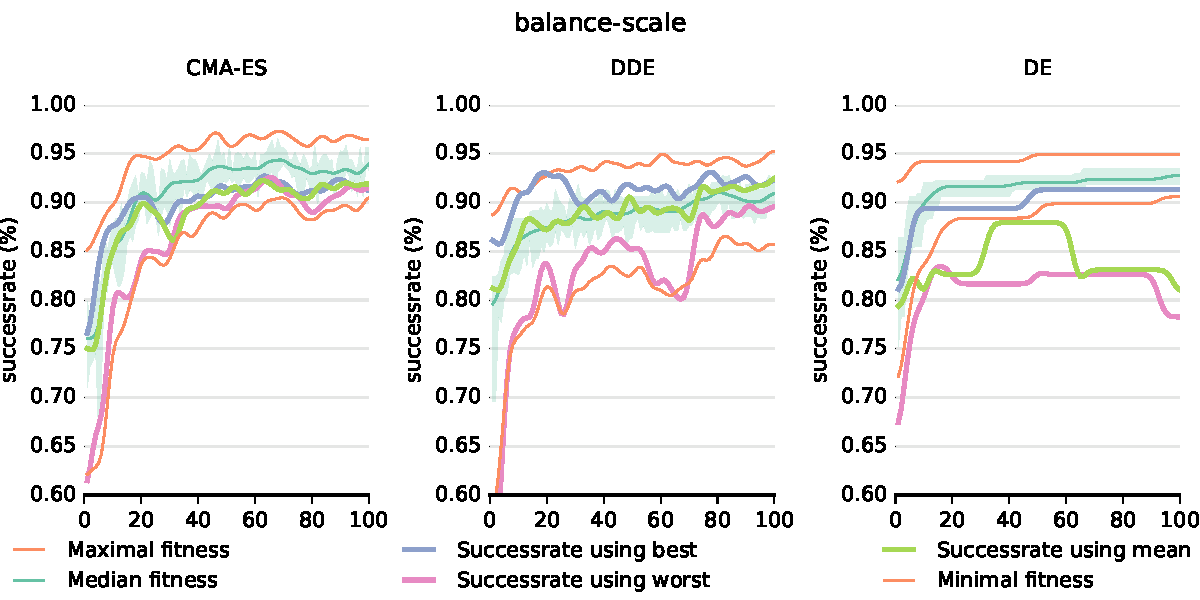
\includegraphics[width=1.0\textwidth]{img/balance-scale}
     %}
     % trim={<left> <lower> <right> <upper>}
     \caption{Logo of MFF UK}
 \end{figure}

% \begin{figure}[ht]
%     \centering
%     \includegraphics[width=1.0\textwidth]{img/dim-reduction/plotly}
%     \caption{Logo of MFF UK}
%     \label{fig:xxx}
% \end{figure}


% Example 1
\ldots when Einstein introduced his formula
\begin{equation}
e = m \cdot c^2 \; ,
\end{equation}
which is at the same time the most widely known
and the least well understood physical formula.
% Example 2
\ldots from which follows Kirchhoff’s current law:
\begin{equation}
\sum_{k=1}^{n} I_k = 0 \; .
\end{equation}
Kirchhoff’s voltage law can be derived \ldots
% Example 3
\ldots which has several advantages.
\begin{equation}
I_D = I_F - I_R
\end{equation}
is the core of a very different transistor model. \ldots

%%%%%%%%%%%%%%%%%%%%%%%%%%%%%%%%%%%%%%%%%%%%%%%%%%%%%%%%%%%%%%%%%%%%%
%%%%%%%%%%%%%%%%%%%%%%%%%%%%%%%%%%%%%%%%%%%%%%%%%%%%%%%%%%%%%%%%%%%%%
%%%%%%%%%%%%%%%%%%%%%%%%%%%%%%%%%%%%%%%%%%%%%%%%%%%%%%%%%%%%%%%%%%%%%

%%% Bibliography
%%% Bibliography (literature used as a source)
%%%
%%% We employ bibTeX to construct the bibliography. It processes
%%% citations in the text (e.g., the \cite{...} macro) and looks up
%%% relevant entries in the bibliography.bib file.
%%%
%%% The \bibliographystyle command selects, which style will be used
%%% for references from the text. The argument in curly brackets is
%%% the name of the corresponding style file (*.bst). Both styles
%%% mentioned in this template are included in LaTeX distributions.

\bibliographystyle{plainnat}    %% Author (year)
% \bibliographystyle{unsrt}     %% [number]

\renewcommand{\bibname}{Bibliography}

%%% Generate the bibliography. Beware that if you cited no works,
%%% the empty list will be omitted completely.

\bibliography{bibliography}

%%% If case you prefer to write the bibliography manually (without bibTeX),
%%% you can use the following. Please follow the ISO 690 standard and
%%% citation conventions of your field of research.

% \begin{thebibliography}{99}
%
% \bibitem{lamport94}
%   {\sc Lamport,} Leslie.
%   \emph{\LaTeX: A Document Preparation System}.
%   2nd edition.
%   Massachusetts: Addison Wesley, 1994.
%   ISBN 0-201-52983-1.
%
% \end{thebibliography}


%%% Figures used in the thesis (consider if this is needed)
\listoffigures

%%% Tables used in the thesis (consider if this is needed)
%%% In mathematical theses, it could be better to move the list of tables to the beginning of the thesis.
\listoftables

%%% Abbreviations used in the thesis, if any, including their explanation
%%% In mathematical theses, it could be better to move the list of abbreviations to the beginning of the thesis.
\chapwithtoc{List of Abbreviations}

%%% Attachments to the master thesis, if any. Each attachment must be
%%% referred to at least once from the text of the thesis. Attachments
%%% are numbered.
%%%
%%% The printed version should preferably contain attachments, which can be
%%% read (additional tables and charts, supplementary text, examples of
%%% program output, etc.). The electronic version is more suited for attachments
%%% which will likely be used in an electronic form rather than read (program
%%% source code, data files, interactive charts, etc.). Electronic attachments
%%% should be uploaded to SIS and optionally also included in the thesis on a~CD/DVD.
\chapwithtoc{Attachments}

\openright
\end{document}
